\documentclass{article}

% Language setting
% Replace `english' with e.g. `spanish' to change the document language
\usepackage[english]{babel}

% Set page size and margins
% Replace `letterpaper' with `a4paper' for UK/EU standard size
\usepackage[letterpaper,top=2cm,bottom=2cm,left=3cm,right=3cm,marginparwidth=1.75cm]{geometry}

% Useful packages
\usepackage{amsmath}
\usepackage{graphicx}
\usepackage[colorlinks=true, allcolors=blue]{hyperref}

\title{Git Tutorial}
\author{Nico Cantrell}

\begin{document}
\maketitle

\section{Introduction}

This tutorial will focus on explaining git using the Github Desktop application as an example.

\section{What is Git?}

    Git is a version control system widely used in software development. When developing programs, especially with multiple people, keeping track of files and retaining the history of those files is essential. Version control systems provide a solution to this problem. The version control system records every version of every file in something called a repository so that history can always be accessed.

\section{Cloning a Repository}

    In order to work on project with multiple people at the same time, each user clones the repository, creating a local copy on their machine that they can work on. This local version of the repository is called a working copy and all edits made on the working copy only affect your version of the repository.    

\section{Commits}

    The user can edit their local copy as much as they would like but when they are ready to save their work to the history of the project they have to make a commit. Commits are a formal checking in of the current state of the files to the local copy of the repository. Each commit has a log message associated with it so that it is clear what changes were made when looking back at the history. Commits can also be assigned tags that give more information about each commit and make the history easier to parse. Tags can be useful to assign versions to commits and are often tagged with release versions.

\section{Pushing and pulling}

    Pushing allows you to move the changes present on your local copy to the remote repository. When you push it updates the remote repository with all commits that have happened since your last push. You can only push to the remote repository when you have all commits present on the remote repository on your local copy. If someone else has pushed to the remote repository, you will have to pull changes before you push. Pulling code that does not match your local copy can create merge conflicts, which we cover later.
    
\section{Branches}

    Branches are different versions of the repository that allow users to work on different versions of the files. This can be useful to try out creating new features without breaking the code for everyone else working on the project. Generally, there is one "main" branch that is the most recent version of the code that works. 

\section{Stashes}

    When you want to switch over to another branch but you have changes that you have not committed yet, the uncommitted changes are "stashed". This allows you to work on a different branch or check on the status of a different branch without having to commit unfinished changes. You can only have one set of stashed changes at a time, and if you try to stash a new set you have to either discard them or overwrite the previous stash.
    
\section{Merging}

    When you want to add the changes made in a branch, (for example: feature-branch), to another branch, (for example: main-branch), you can "merge" the two branches together. Merging attempts to copy all the changes made in the feature-branch to the main-branch, adding in any extra code that is present in feature-branch to main-branch.

\section{Merge Conflicts}

    When the differences in two files are too significant to automatically combine, a merge conflict is created. For example, these are two versions of the same file:
\begin{figure}
    \centering
    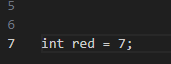
\includegraphics[width=0.5\linewidth]{image.png}
    \caption{feature branch}
    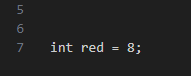
\includegraphics[width=0.5\linewidth]{File2.png}
    \caption{main branch}
\end{figure}
When attempting to merge this file between the two branches, git cannot decide which version of the file to use and you will have to resolve this conflict by picking one version of line 7 to be in the merged file. 

\section{Getting Started}

Let's start by installing GitHub desktop.  Go to \href{https://desktop.github.com/}{https://desktop.github.com/} and install the version for your operating system.  Unzip the files and run the program. Next GitHub will ask you to sign in to your GitHub account. If you do not have one create one, otherwise sign in to your account.

    To start our tutorial, on the next screen select "clone a repository from the internet." Enter the url: nzwt/GithubTutorial. Now you have a local copy of the GithubTutorial repository. Your screen should look like this:
    \begin{figure}
        \centering
        
\begin{figure}
            \centering
            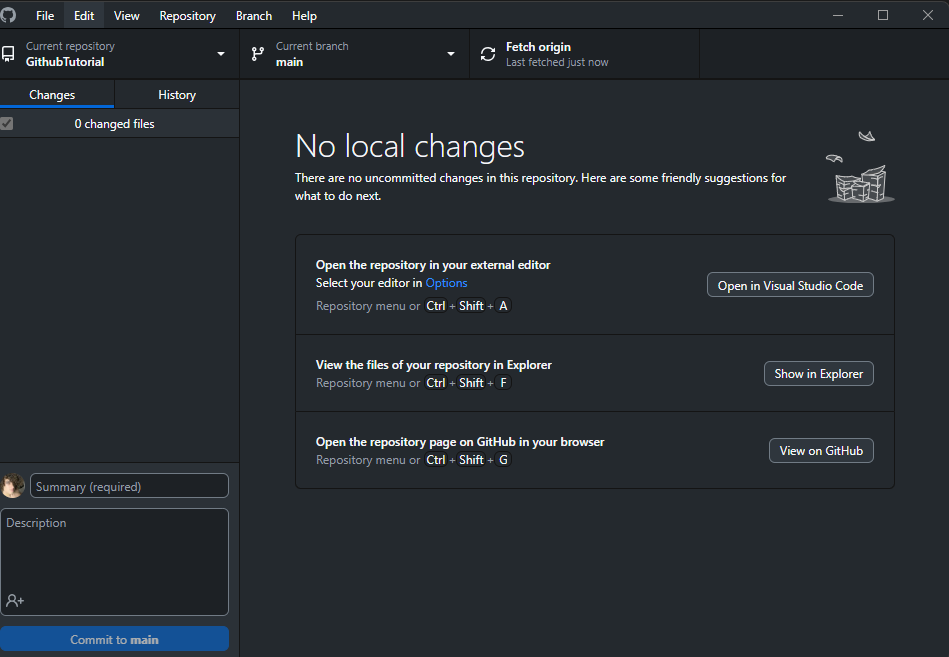
\includegraphics[width=1\linewidth]{MainScreen.png}
        \end{figure}
        
        
    \end{figure}

    Let's go through the options on this main page and explain what they mean:
    \begin{itemize}
        \item Current repository:
\begin{figure}
    \centering
    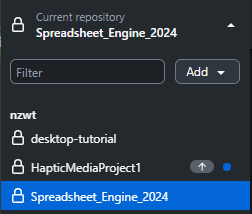
\includegraphics[width=0.5\linewidth]{repositories.png}
\end{figure}
        \begin{itemize}
                \item This allows you to select the repository you are currently working on. Different projects often have different repositories, so this allows you to switch between projects. 
                \item Selecting add gives you the option to clone new repositories not present on your local machine from their url or repositories that you have added to your github account.


        \end{itemize}
        \item Current branch:
\begin{figure}
    \centering
    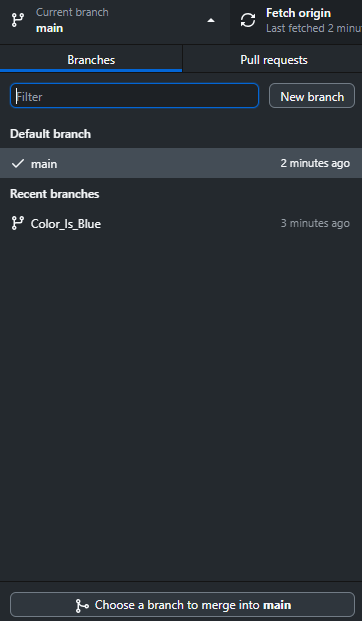
\includegraphics[width=0.5\linewidth]{branches.png}
    \caption{Branches}
\end{figure}
        \begin{itemize}
            \item This allows you to switch between branches available in the repository
            \item This is an example of a project with several different branches. By selecting a different branch the files on your computer will be updated to match the files on the branch.
            \item This is also where you can initiate merges of branches, which will be covered later.
        \end{itemize}
    \end{itemize}

\section{Making a commit}

    Try editing welcome.txt with whatever text you want. When you are done editing and ready to commit your changes, go back to GitHub desktop.
    \begin{figure}
        \centering
        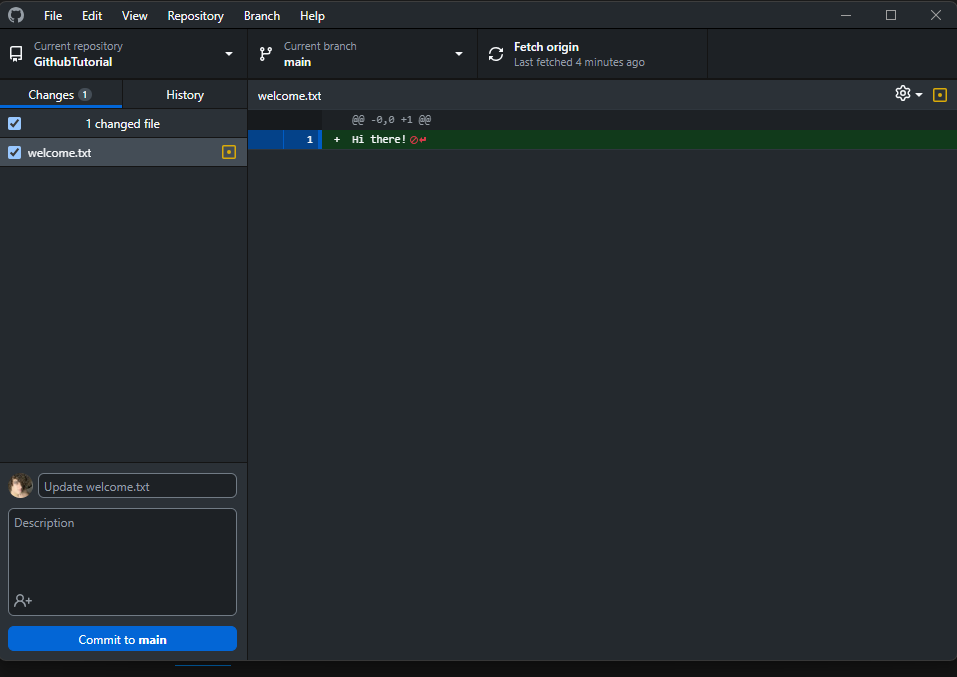
\includegraphics[width=1\linewidth]{commit.png}
    \end{figure}
    The changes tab in the left will show all files that you have made changes to. files that are checked will be included in the commit and files unchecked will not be committed. In the bottom left GitHub will suggest a commit message, here "Update welcome.txt" but you should replace this commit message with something more descriptive. The description can be used to further specify what changes you made and help others (or yourself) understand what you did in the future.

\section{Pushing and Pulling}

    Before we push we want to make sure that we have the most up to date version of the repository. In order to do this, press the "fetch origin" button on the top left. If changes are available to pull this option will change to "Pull origin." Once you have pulled all changes and made a commit you are ready to push! After you make a commit, the "fetch origin" button will change to a "push origin" button that will push your changes to the remote repository.

\section{Merge Conflicts}

    To show an example of a merge conflict, on the main branch select the "current branch" button on the top. At the bottom of the branches tab select "Choose a branch to merge to main. Choose the branch "Color_Is_Blue" to merge to main. Selecting this option will display a warning:
    \begin{figure}
        \centering
        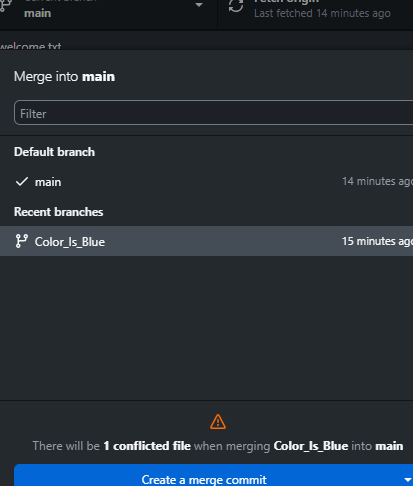
\includegraphics[width=.5\linewidth]{MergeError.png}
    \end{figure}
    Select "Create a merge commit", then open the file in your text editor of choice to resolve the conflict, I am using visual studio code for this process.
    \begin{figure}
        \centering
        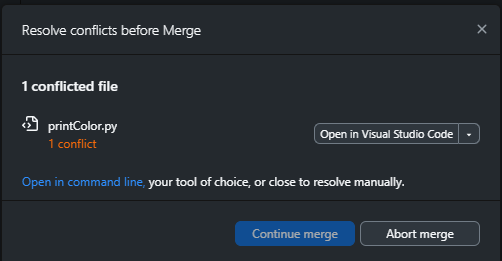
\includegraphics[width=0.5\linewidth]{MergeResolve.png}
    \end{figure}
    This is what the merge conflict file looks like:
    \begin{figure}
        \centering
        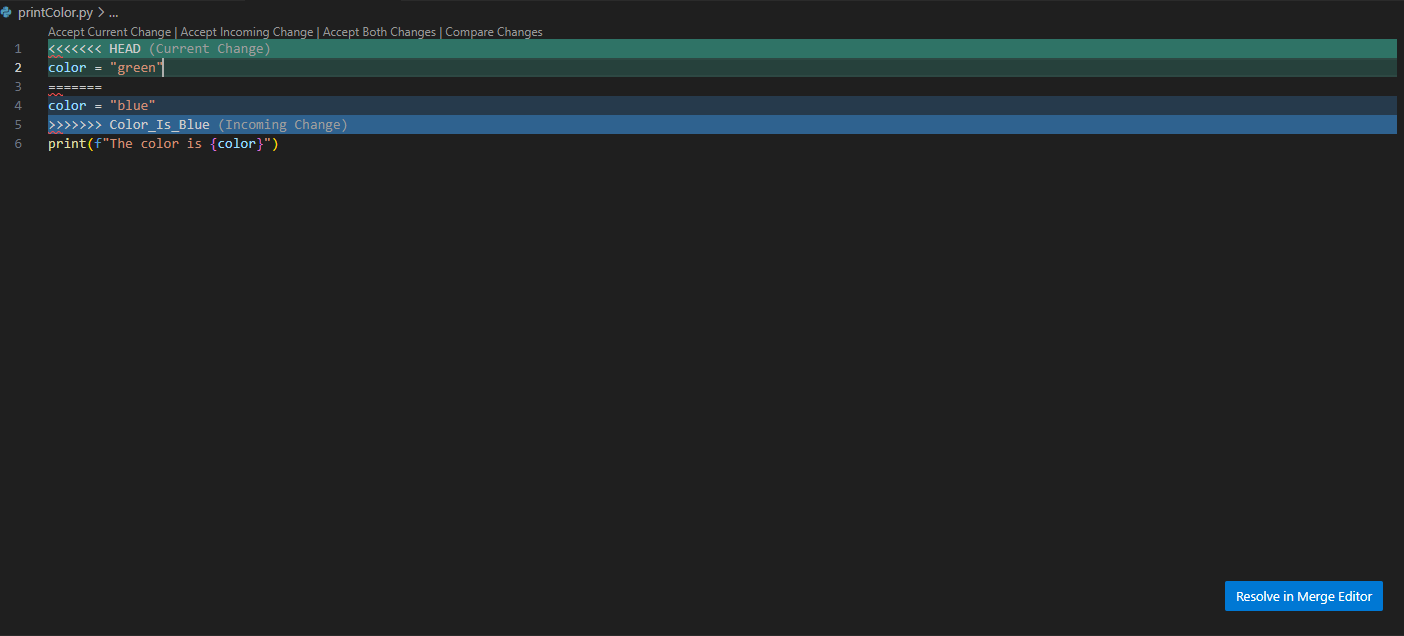
\includegraphics[width=1\linewidth]{MergeConflictFile.png}
    \end{figure}
    HEAD represents the branch we are currently working on (in this case main) and Color_Is_Blue represents the incoming changes we are trying to merge. To resolve the conflict delete the lines that you don't want and leave the lines that you do. In this case if we want to change the color to blue we delete lines 1,2,3 and 5. After editing the file, go back to GitHub desktop where you should see the message "All conflicted files should be resolved."
    \begin{figure}
        \centering
        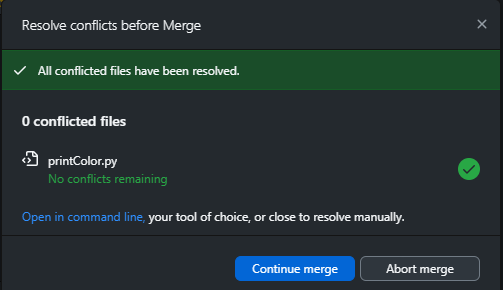
\includegraphics[width=0.5\linewidth]{FilesResolved.png}
    \end{figure}
    Click "continue merge" to formalize the merge and add it as a commit. This merging of branches is listed in history as any other commit and can be pushed and pulled in the same way a regular commit can.

\section{Thank You}

    This tutorial has explained the basics of Git through GitHub desktop. While Git is a powerful tool and can be used for much more complex operations, this tutorial should cover the basics and allow you to contribute to a project.
\end{document}